\documentclass[11pt,a4paper,oneside]{thesis}

\usepackage[utf8]{inputenc}
\usepackage[T1]{fontenc}
\usepackage[english,spanish,es-tabla]{babel}
\usepackage[table,xcdraw]{xcolor}
\usepackage{amsmath,amssymb,amsfonts}
\usepackage{graphicx}
\usepackage{booktabs}
\usepackage{array}
\usepackage{float}
\usepackage{url}
\usepackage{acronym}
\usepackage{csquotes}
\usepackage[backend=bibtex,style=numeric,sorting=none]{biblatex}
\addbibresource{references.bib}

\graphicspath{{figures/}{Figuras/}}
\setlength{\headheight}{26pt}
\hypersetup{colorlinks=false,urlcolor=black}

\thesistitle{Representaciones léxicas y basadas en LLM para la predicción de resultados de licitaciones públicas: un estudio comparativo}
\authors{Isaac Gabriel Amarilla Benítez y Luis Fernando Caballero Ramoa}
\degree{Ingeniería en Informática}
\subject{Predicción de resultados de licitaciones públicas mediante representaciones textuales}
\keywords{contratación pública, documentos de licitación, modelos de lenguaje, predicción de resultados}
\university{Universidad Nacional de Asunción}
\UNIVERSITY{UNIVERSIDAD NACIONAL DE ASUNCIÓN}
\faculty{Facultad Politécnica}
\FACULTY{FACULTAD POLITÉCNICA}
\department{Ingeniería en Informática}
\DEPARTMENT{INGENIERÍA EN INFORMÁTICA}

\begin{document}
\selectlanguage{spanish}
\renewcommand{\listtablename}{Lista de tablas}
\renewcommand{\bibname}{Referencias}
\renewcommand{\listfigurename}{Lista de figuras}
\renewcommand{\contentsname}{Contenidos}

\frontmatter
\setstretch{1.3}
\fancyhead{}
\rhead{\thepage}
\pagestyle{fancy}

\begin{titlepage}
  \begin{center}
    \vspace*{-1.2in}
    {\fontsize{14}{15}\bfseries UNIVERSIDAD NACIONAL DE ASUNCIÓN\par}
    \vspace{0.5cm}
    {\fontsize{12}{15}\bfseries FACULTAD POLITÉCNICA\par}
    \vspace{0.15in}
    INGENIERÍA EN INFORMÁTICA
    \vspace{0.25in}

    
\includegraphics[width=7cm,height=8cm,keepaspectratio]{Figuras/fpuna_logo_institucional.png}

    \vspace{0.15in}
    {\Large\bfseries REPRESENTACIONES LÉXICAS Y BASADAS EN LLM PARA LA PREDICCIÓN DE RESULTADOS DE LICITACIONES PÚBLICAS: UN ESTUDIO COMPARATIVO\par}
    \vspace{0.3in}
    {\large Proyecto Final de Grado\par}
    \vspace{0.35in}
    {\bfseries Autores:}\par
    Isaac Gabriel Amarilla Benítez\par
    Luis Fernando Caballero Ramoa\par
    \vfill
    {\large San Lorenzo -- Paraguay\par}
    \vspace{0.2in}
    {\large\bfseries 2026\par}
  \end{center}
\end{titlepage}

\clearpage
\begin{abstract}
\addcontentsline{toc}{chapter}{Abstract}
We compare lexical and LLM-based text representations for predicting public tender outcomes from bidding documents in a processed subset of 1{,}162 road-construction procurements (Paraguay). Under stratified 5-fold cross-validation, TF--IDF with logistic regression yields the strongest ranking (mean ROC AUC 0.814, PR AUC 0.899), while a lightweight cross-chunk transformer over frozen LLM chunk embeddings achieves the best calibration (Brier 0.162) and the most stable behavior under threshold tuning. The study highlights that procurement documents carry ex ante predictive signal and that ranking, calibration, and threshold sensitivity should be assessed separately for monitoring. Artifacts: doi:10.5281/zenodo.20128769.
\end{abstract}

\clearpage
\begin{resumen}
\addcontentsline{toc}{chapter}{Resumen}
Este trabajo compara representaciones textuales léxicas y basadas en LLM para predecir resultados de licitaciones públicas a partir de documentos de licitación en un subconjunto procesado de 1.162 contrataciones de construcción vial de Paraguay. Bajo validación cruzada estratificada de cinco pliegues, TF--IDF con regresión logística produce el mejor ordenamiento, con ROC AUC medio de 0,814 y PR AUC de 0,899, mientras que un transformer liviano entre fragmentos, aplicado sobre embeddings congelados de fragmentos de un LLM, logra la mejor calibración, con un puntaje de Brier de 0,162, y el comportamiento más estable ante el ajuste del umbral. El estudio destaca que los documentos de contratación contienen señal predictiva temprana y que el ordenamiento, la calibración y la sensibilidad al umbral deben evaluarse por separado para el monitoreo. Artefactos: doi:10.5281/zenodo.20128768.

\textbf{Palabras clave:} contratación pública, gobierno electrónico, democracia electrónica, documentos de licitación, pliego de bases y condiciones, modelos grandes de lenguaje, predicción de resultados.
\end{resumen}


\clearpage
\pagestyle{fancy}
\lhead{\emph{Contenidos}}
\setcounter{tocdepth}{3}
\tableofcontents
\clearpage
\lhead{\emph{Lista de figuras}}
\listoffigures
\clearpage
\lhead{\emph{Lista de tablas}}
\listoftables
\clearpage
\lhead{\emph{Glosario}}
\chapter*{Glosario}
\addcontentsline{toc}{chapter}{Glosario}
\section*{Acrónimos}
\begin{acronym}[TF--IDF]
  \setlength{\itemsep}{0pt}
  \setlength{\parskip}{0pt}
  \acro{API}{\textit{Application Programming Interface}}
  \acro{AUC}{\textit{Area Under the Curve}}
  \acro{CV}{\textit{Cross-Validation}}
  \acro{DNCP}{Dirección Nacional de Contrataciones Públicas}
  \acro{GPU}{\textit{Graphics Processing Unit}}
  \acro{LLM}{\textit{Large Language Model}}
  \acro{MLP}{\textit{Multilayer Perceptron}}
  \acro{OCDE}{Organización para la Cooperación y el Desarrollo Económicos}
  \acro{OCDS}{\textit{Open Contracting Data Standard}}
  \acro{OCR}{\textit{Optical Character Recognition}}
  \acro{PBC}{Pliego de Bases y Condiciones}
  \acro{PR}{\textit{Precision--Recall}}
  \acro{ROC}{\textit{Receiver Operating Characteristic}}
  \acro{SICP}{Sistema de Información de las Contrataciones Públicas}
  \acro{TFIDF}[TF--IDF]{\textit{Term Frequency--Inverse Document Frequency}}
\end{acronym}

\section*{Términos}
\begin{description}
  \setlength{\itemsep}{0.15\baselineskip}
  \setlength{\parskip}{0pt}
  \item[Agregación por promedio:] operación que resume varios embeddings mediante su media aritmética para obtener una única representación.
  \item[Calibración:] grado de correspondencia entre las probabilidades predichas y las frecuencias observadas de un resultado.
  \item[Clasificación binaria:] tarea de asignar cada ejemplo a una de dos clases posibles.
  \item[Codificador congelado:] modelo preentrenado cuyos parámetros no se actualizan durante el entrenamiento del predictor posterior.
  \item[Detención temprana:] criterio que interrumpe el entrenamiento cuando el desempeño de validación deja de mejorar durante un número prefijado de épocas.
  \item[Embedding:] representación vectorial densa de una unidad textual, producida por un modelo para codificar regularidades de su contenido y contexto.
  \item[Época:] recorrido completo del algoritmo de entrenamiento sobre todos los ejemplos de la partición destinada al ajuste.
  \item[Fragmento:] segmento de tokens en el que se divide un documento para respetar el límite de entrada del codificador.
  \item[Fuga de información:] uso durante el entrenamiento o la selección de información que no estaría disponible en el momento real de la predicción.
  \item[Hiperparámetro:] valor fijado antes del entrenamiento que controla la configuración o el comportamiento de un modelo.
  \item[Logit:] salida numérica de un clasificador antes de transformarla en probabilidad mediante una función como la sigmoide.
  \item[$n$-grama:] secuencia contigua de $n$ unidades de texto. En este trabajo las unidades son palabras: un unigrama contiene una palabra y un bigrama contiene dos.
  \item[Ordenamiento:] capacidad de asignar puntajes mayores a los ejemplos positivos que a los negativos, independientemente de un umbral fijo.
  \item[Prevalencia:] proporción de ejemplos pertenecientes a la clase positiva dentro de un conjunto de datos.
  \item[Representación densa:] vector numérico en el que la información se distribuye entre un número fijo de componentes, generalmente no nulas.
  \item[Representación dispersa:] vector de alta dimensión en el que la mayoría de los componentes son cero, como una representación TF--IDF.
  \item[Token:] unidad mínima de texto procesada por un tokenizador; puede corresponder a una palabra, parte de ella o un símbolo.
  \item[Transformer:] arquitectura neuronal basada principalmente en mecanismos de atención para modelar relaciones entre elementos de una secuencia.
  \item[Umbral de decisión:] valor de corte aplicado a un puntaje o probabilidad para convertirlo en una predicción de clase.
  \item[Validación cruzada:] procedimiento que divide los datos en varios pliegues y alterna cuáles se usan para entrenamiento y evaluación.
\end{description}


\mainmatter
\selectlanguage{spanish}
\pagestyle{fancy}
\chapter{Introducción}
La contratación pública es un proceso central del gobierno electrónico: transforma los presupuestos públicos en contratos, obras y servicios mediante plataformas cada vez más digitales. También es relevante para la democracia electrónica, porque los registros abiertos de contratación amplían la capacidad de los organismos de control, periodistas, empresas y ciudadanos para examinar cómo se asignan los recursos públicos. Estas capacidades se alinean con las agendas de gobierno digital sobre datos abiertos y análisis responsables para la supervisión del sector público. Trabajos recientes en este sector presentan el análisis de contrataciones como una herramienta para la supervisión basada en riesgos \cite{salazar2024vigia}. Los documentos de licitación son fundamentales en este contexto porque definen las condiciones administrativas, los requisitos técnicos, las reglas de calificación y las restricciones de ejecución antes de que se conozca el resultado final. Evidencia reciente del ámbito de las contrataciones también muestra que las descripciones de las convocatorias permiten predecir resultados relacionados con la competencia y la eficiencia de costos \cite{acikalin2024procurementcalls}. Por tanto, la pregunta relevante no es solo si los resultados de las licitaciones pueden predecirse a partir del texto documental, sino también qué representación de ese texto aporta más información para un monitoreo responsable de la contratación pública.

Este trabajo estudia dicha pregunta mediante una comparación directa entre características léxicas dispersas y representaciones densas basadas en LLM. El análisis se concentra en licitaciones de construcción vial, cuyos documentos suelen ser relativamente estructurados y estandarizados. Los modelos léxicos dispersos continúan siendo líneas base sólidas e interpretables para la clasificación documental \cite{wang2012baselines}, y trabajos recientes sobre documentos extensos confirman que las representaciones léxicas o híbridas pueden seguir siendo competitivas, en lugar de quedar uniformemente superadas por arquitecturas transformer \cite{alvaprincipe2025survey}. Al mismo tiempo, la investigación sobre embeddings se ha extendido hacia representaciones densas basadas en LLM \cite{wang2024improvingembeddings}. En este contexto, el objetivo no es establecer una familia de modelos universalmente superior, sino comprender cuánta señal predictiva puede recuperarse de indicios léxicos, cuánta ya está capturada por embeddings densos congelados y si el modelado explícito de interacciones entre fragmentos aporta valor adicional.

La canalización utiliza un LLM causal preentrenado como codificador congelado para producir embeddings por fragmento a partir de documentos de licitación en español. Se comparan dos estrategias simples de agregación de estos embeddings, basadas en agrupación por promedio, con un transformer liviano que modela las interacciones entre fragmentos. Estos enfoques basados en LLM se evalúan junto con TF--IDF más regresión logística y líneas base triviales. Este diseño permite separar los efectos de la representación de los efectos del modelado posterior.

El estudio ofrece una comparación reproducible entre líneas base léxicas, triviales, de embeddings agregados y de un transformer entre fragmentos, bajo validación cruzada determinista de cinco pliegues. También analiza por separado el desempeño de ordenamiento, la calibración y la sensibilidad al umbral. El resultado central presenta matices: TF--IDF más regresión logística es el modelo con mejor ordenamiento, mientras que el transformer entre fragmentos ofrece la mejor calibración y el comportamiento más estable ante cambios del umbral. Esto aporta evidencia útil para la pregunta más amplia de cómo se distribuye la señal textual en los documentos de contratación pública. Los artefactos asociados están archivados en Zenodo (doi:10.5281/zenodo.20128769).

\chapter{Definición de la tarea}
La tarea de predicción consiste en una clasificación binaria sobre contrataciones para las cuales se dispone tanto de un documento de licitación utilizable como de una etiqueta de resultado. Cada ejemplo corresponde a un proceso de contratación emparejado con un documento PBC extraído. La variable objetivo se operacionaliza a partir del campo de estado de la contratación de la siguiente manera:

\begin{itemize}
  \item Resultado exitoso ($y=1$): \texttt{complete}.
  \item Resultado no exitoso ($y=0$): \texttt{unsuccessful}, \texttt{cancelled} o \texttt{canceled}.
\end{itemize}

Los registros con otros estados se excluyen del entrenamiento supervisado y de la evaluación. Esta definición es intencionalmente simple y se fundamenta directamente en la fuente de datos disponible. Debe entenderse como una aproximación operativa al éxito de una contratación y no como una noción institucional exhaustiva de desempeño.

\chapter{Método}
\section{Representación documental}
Cada documento PBC se convierte primero de PDF a texto mediante la canalización de extracción previa. El texto resultante se tokeniza y divide en fragmentos superpuestos. En la implementación actual, cada fragmento tiene una longitud de 4096 tokens y un desplazamiento de 2048 tokens. Se utiliza el modelo de lenguaje causal preentrenado \texttt{openai/gpt-oss-20b} como codificador documental congelado \cite{agarwal2025gptoss}. Este modelo se seleccionó como un LLM práctico de pesos abiertos para extraer representaciones densas de textos de contratación en español y, a la vez, mantener reproducible la canalización experimental. Congelar el codificador también evita ajustar un modelo grande sobre un conjunto de datos modesto y permite que la comparación se concentre en cuánta señal existe en las representaciones preentrenadas y cómo se agrega posteriormente, en consonancia con trabajos recientes sobre embeddings textuales basados en LLM \cite{wang2024improvingembeddings}. Los fragmentos se procesan en microlotes para reducir la presión sobre la memoria de la GPU.

Para cada fragmento, el sistema extrae la representación oculta asociada al último token válido. La salida correspondiente a un documento de contratación es, por tanto, una secuencia de embeddings de fragmentos:
\[
\mathbf{E} = [\mathbf{e}_1, \mathbf{e}_2, \dots, \mathbf{e}_N], \qquad \mathbf{e}_i \in \mathbb{R}^{d_{in}},
\]
donde $N$ es la cantidad de fragmentos del documento y $d_{in}$ está determinado por el tamaño oculto del modelo preentrenado. Esta configuración permite comparar dos estrategias de representación basadas en LLM: un vector documental simple obtenido mediante el promedio de los fragmentos y un modelo secuencial que aprende las interacciones entre ellos.

\section{Arquitectura del predictor}
El clasificador principal, \texttt{TenderSuccessPredictor}, es un transformer liviano aplicado sobre los embeddings de los fragmentos. Sea $\mathbf{E} \in \mathbb{R}^{N \times d_{in}}$ la secuencia de fragmentos de un documento. El modelo aplica:

\begin{enumerate}
  \item Una proyección lineal de $d_{in}$ a una dimensión latente entrenable $d_{model}$.
  \item La inserción de un token aprendido \texttt{[CLS]} al comienzo de la secuencia.
  \item Un codificador transformer sobre la secuencia completa de vectores de fragmentos.
  \item Una pequeña cabeza de clasificación multicapa sobre la representación final de \texttt{[CLS]}.
\end{enumerate}

En los experimentos actuales, los hiperparámetros posteriores son: $d_{model}=128$, $n_{heads}=4$, dimensión de la red prealimentada $=512$, dropout $=0.3$ y una capa de codificación. Se emplean máscaras de relleno para agrupar de forma segura documentos con diferentes cantidades de fragmentos.

El modelo produce un único logit por documento. Una transformación sigmoide convierte este logit en una probabilidad de éxito:
\[
\hat{p}(y=1 \mid \mathbf{E}) = \sigma(z).
\]
El entrenamiento utiliza entropía cruzada binaria con logits.

\section{Líneas base}
Para interpretar los resultados basados en LLM, se evalúan tres clases de líneas base.

En primer lugar, se emplean dos referencias triviales: un clasificador de clase mayoritaria y un clasificador aleatorio cuya tasa positiva coincide con la prevalencia empírica. Estas líneas base establecen la región esperada sin capacidad predictiva, donde ROC AUC debería situarse cerca de $0.5$ y PR AUC cerca de la prevalencia positiva.

En segundo lugar, se utiliza una línea base léxica con características TF--IDF de hasta 50.000 unigramas y bigramas, frecuencia documental mínima de $5$ y un clasificador de regresión logística con pesos de clase balanceados. Se utiliza TF--IDF en lugar de embeddings densos estáticos como Word2Vec porque proporciona una referencia sólida e interpretable de bolsa de palabras que sigue siendo competitiva en documentos extensos \cite{wang2012baselines,alvaprincipe2025survey}. Además, permite aislar la comparación con representaciones congeladas de LLM sin añadir otra etapa entrenable de embeddings bajo supervisión limitada. Las líneas base lineales de bolsa de palabras son referencias habituales en clasificación de textos \cite{wang2012baselines}, y la evidencia reciente sobre documentos extensos indica que las representaciones léxicas aún son competitivas en algunos escenarios \cite{alvaprincipe2025survey}.

En tercer lugar, se definen dos líneas base intermedias basadas en LLM que utilizan los mismos embeddings preentrenados de fragmentos que el sistema principal, pero sustituyen el transformer entre fragmentos por una agregación documental más simple. En la primera variante, se promedian los embeddings de los fragmentos y se suministran a una regresión logística. En la segunda, la misma representación promedio alimenta un pequeño perceptrón multicapa con una capa oculta. Estas líneas base aíslan el valor de la representación del valor aportado por el modelado explícito de las interacciones entre fragmentos.

\section{Entrenamiento y reproducibilidad}
El entrenamiento utiliza AdamW, una tasa de aprendizaje de $10^{-4}$, decaimiento de pesos de $0.01$, lotes de tamaño $8$ y hasta $50$ épocas. Dentro de cada ronda de validación cruzada, una época corresponde a un recorrido completo por la porción de entrenamiento de esa ronda. Después de cada época se calcula la pérdida de validación sobre la porción reservada; si no mejora durante cinco épocas consecutivas, el entrenamiento se detiene y se restaura el mejor punto de control. La reproducibilidad se controla mediante semillas fijas, comportamiento determinista de cuDNN, cargadores de datos con semilla y reinicios independientes del estado aleatorio al comienzo de cada pliegue.

\chapter{Configuración experimental}
\section{Conjunto de datos}
La instantánea de metadatos utilizada en este trabajo se construyó a partir de registros de contratación pública publicados por la Dirección Nacional de Contrataciones Públicas (DNCP) de Paraguay y recuperados mediante el endpoint oficial de datos abiertos \texttt{v3/doc/search/processes}. El conjunto inicial contiene 10.628 contrataciones de construcción vial bajo el código de catálogo \texttt{72131701}: 10.000 procesos completados materializados por una canalización previa de extracción de la DNCP y 628 procesos adicionales no exitosos recolectados según su estado. Para reducir el desbalance de clases, la recuperación y el procesamiento priorizaron las contrataciones no exitosas antes que las completadas.

El subconjunto supervisado es menor porque se requieren varios pasos de filtrado. La mayor reducción ocurre antes del procesamiento textual: solo se recuperaron 1.845 PDF de PBC, principalmente porque los límites de solicitudes de la DNCP impidieron realizar una búsqueda y descarga exhaustivas dentro del tiempo disponible. Luego, la canalización extrajo texto de 1.842 PDF y generó embeddings congelados del LLM para 1.162 documentos. Los tres fallos de extracción correspondieron a documentos escaneados no compatibles con el extractor sin OCR, mientras que la mayoría de los fallos de generación de embeddings fueron errores por falta de memoria en la GPU, después de una única ejecución limitada por el costo de infraestructura. Por ello, las conclusiones se aplican a este subconjunto procesado y no automáticamente a toda la población de contrataciones.

La distribución de clases del subconjunto procesado presenta un desbalance moderado: 844 contrataciones ($72.63\%$) están etiquetadas como exitosas (\texttt{complete}) y 318 ($27.37\%$) como no exitosas (\texttt{unsuccessful}/\texttt{cancelled}/\texttt{canceled}). La longitud media representada es de 7,46 fragmentos por contratación, con una desviación estándar de 13,52, una mediana de 3 fragmentos y un máximo de 245. Estos valores indican una distribución de longitudes muy asimétrica, con numerosos documentos cortos y una cantidad menor de documentos considerablemente más largos. La dimensión de los embeddings heredada del LLM base congelado es 2880.

El subconjunto procesado también está menos desbalanceado que la población general de contrataciones. En la instantánea completa, los resultados exitosos son mucho más frecuentes: aproximadamente 10.000 contrataciones exitosas frente a unas 650 no exitosas. Por consiguiente, las métricas dependientes del umbral y las interpretaciones sensibles a la prevalencia deben considerarse válidas para el subconjunto procesado, no como puntos operativos directamente desplegables.

\section{Tratamiento de la fuga de información}
El modelo opera exclusivamente con información disponible en el momento de la inferencia. Todas las entradas se derivan de documentos de licitación producidos y publicados durante la etapa de convocatoria, antes de que se conozca el resultado final de la contratación. Esto hace que la configuración predictiva sea operativamente realista y reduce sustancialmente el riesgo de fuga directa a partir de contenido explícito sobre el estado final.

En consecuencia, la principal amenaza restante para la validez no es una fuga evidente y posterior de la variable objetivo, sino las correlaciones predictivas indirectas y la representatividad limitada. Los documentos de licitación pueden codificar regularidades estructurales, institucionales o estilísticas que predicen el resultado sin ser causales. Estas regularidades son legítimas para la predicción ex ante porque están disponibles en el momento de la decisión, pero no deben interpretarse como causas directas del éxito o fracaso de una contratación.

\section{Protocolo de evaluación}
El modelo se evalúa mediante validación cruzada estratificada de cinco pliegues. El subconjunto procesado de 1.162 ejemplos se divide en cinco pliegues que preservan las etiquetas, de modo que cada ronda utiliza aproximadamente cuatro quintas partes de los datos para ajustar el modelo y una quinta parte como partición de evaluación fuera de pliegue. En términos concretos, cada ronda entrena con unas 930 contrataciones y evalúa aproximadamente 232 que no se utilizaron para ajustar el modelo de esa ronda.

La estratificación es importante porque la clase positiva no está balanceada: cerca del $72.6\%$ del subconjunto procesado corresponde a resultados exitosos. Conservar esta prevalencia entre pliegues reduce variaciones evitables en F1, exactitud balanceada y PR AUC. Los valores finales informados son la media y la desviación estándar de los cinco pliegues reservados. Para el análisis de sensibilidad al umbral, los cuatro pliegues de entrenamiento de cada ronda se dividen nuevamente en una porción interna de entrenamiento y otra de validación; el umbral que maximiza F1 en la validación interna se aplica después al pliegue de evaluación externo de esa ronda.

\section{Métricas}
La evaluación utiliza las siguientes métricas:

\begin{itemize}
  \item \textbf{ROC AUC}, para medir la calidad del ordenamiento con independencia del umbral de decisión.
  \item \textbf{PR AUC} (precisión promedio), para evaluar el ordenamiento con atención explícita a la clase positiva.
  \item \textbf{Puntaje F1}, con un umbral de probabilidad de $0.5$.
  \item \textbf{Exactitud balanceada}, también con un umbral de $0.5$.
  \item \textbf{Puntaje de Brier}, para medir la calidad de la calibración probabilística.
  \item \textbf{Pérdida logarítmica}, como regla de puntuación propia sobre las probabilidades predichas.
\end{itemize}

La elección de métricas ante el desbalance depende del objetivo operativo: los resúmenes basados en PR enfatizan la recuperación de la clase positiva, mientras que ROC AUC y PR AUC responden de manera distinta a la prevalencia y deben interpretarse en contexto \cite{richardson2024roc}. Debido a que PR AUC puede inducir a error cuando la clase positiva es frecuente, se interpreta junto con la prevalencia positiva $\pi$ en los pliegues reservados. La implementación también registra \texttt{positive\_prevalence} y \texttt{pr\_auc\_excess\_over\_prevalence}; esta última se define como PR AUC menos $\pi$. La cantidad ofrece una estimación compacta de cuánto mejora el modelo sobre la frecuencia de la clase positiva, utilizada habitualmente como referencia al discutir el comportamiento PR sin capacidad predictiva en contextos desbalanceados.

\chapter{Resultados}
\section{Desempeño de ordenamiento}
La Tabla~\ref{tab:main-results} resume la comparación de modelos. Las líneas base triviales se comportan como se esperaba: ROC AUC permanece en el nivel del azar y PR AUC se mantiene cerca de la prevalencia positiva de aproximadamente $0.726$. Esto proporciona una referencia útil sin capacidad predictiva y respalda la consistencia interna de la evaluación.

Entre los modelos no triviales, TF--IDF más regresión logística obtiene las mejores métricas de ordenamiento, con ROC AUC medio de $0.814$ y PR AUC medio de $0.899$. El transformer entre fragmentos aplicado a embeddings de LLM alcanza ROC AUC de $0.755$ y PR AUC de $0.886$. Las líneas base con embeddings promediados se mantienen próximas: el MLP con promedio alcanza ROC AUC de $0.763$ y PR AUC de $0.894$, mientras que la regresión logística con promedio alcanza ROC AUC de $0.758$ y PR AUC de $0.881$. La Fig.~\ref{fig:pr} coincide con este panorama: TF--IDF define en general la mejor frontera entre precisión y exhaustividad, mientras que ambas alternativas basadas en LLM permanecen claramente por encima de la prevalencia. Los documentos contienen señal predictiva, pero el mejor ordenamiento en la configuración actual proviene de representaciones léxicas y no densas.

\section{Sensibilidad al umbral}
El comportamiento dependiente del umbral revela un patrón diferente. Con el umbral predeterminado de $0.5$, el transformer entre fragmentos alcanza el mayor F1 ($0.858$ en la evaluación original de cinco pliegues). Sin embargo, el experimento específico muestra que no todos los modelos reaccionan de igual manera a la optimización del umbral. Para TF--IDF más regresión logística, seleccionar en validación el umbral que maximiza F1 incrementa el F1 del pliegue de prueba en $0.103$ en promedio, pero no mejora la exactitud balanceada media. La regresión logística con promedio presenta una mejora modesta de F1 ($+0.014$) y una disminución media de exactitud balanceada ($-0.049$). En contraste, el transformer cambia poco con el ajuste (media de $\Delta$F1 $=+0.002$ y media de $\Delta$ de exactitud balanceada $=+0.002$), lo que indica que el umbral predeterminado ya está cerca de un punto operativo estable. El MLP con promedio ocupa una posición intermedia: su F1 apenas cambia, pero su exactitud balanceada mejora en promedio al ajustar el umbral. La Fig.~\ref{fig:threshold-sensitivity} resume visualmente el contraste y deja claro que la optimización beneficia principalmente el F1 del modelo léxico, no a todos los modelos de manera uniforme.

\section{Calibración}
La calibración presenta una historia diferente al ordenamiento. El transformer entre fragmentos consigue el mejor puntaje de Brier ($0.162$), seguido por el MLP con promedio ($0.165$); TF--IDF más regresión logística obtiene un resultado inferior ($0.179$) y la regresión logística con promedio es considerablemente peor ($0.201$). Este patrón indica que las características léxicas pueden ser muy eficaces para ordenar ejemplos, mientras que las representaciones densas basadas en LLM proporcionan probabilidades más confiables. La Fig.~\ref{fig:calibration} concuerda con esta interpretación: entre las tres familias más informativas, el transformer permanece más próximo a la diagonal en gran parte del intervalo de probabilidades, mientras que TF--IDF es mejor en ordenamiento que en calibración. Esto importa porque la selección de modelos para monitorear contrataciones puede depender no solo del ordenamiento, sino también de si las probabilidades permiten sustentar la priorización posterior o una puntuación de riesgo \cite{silvafilho2023calibration}.

\section{Comparación de representaciones}
La comparación entre embeddings promediados y el transformer entre fragmentos es informativa por sí misma. Si el valor principal de la representación del LLM proviniera únicamente de las interacciones entre fragmentos, cabría esperar que el transformer dominara las líneas base con promedio. Esto no sucede. El MLP con promedio supera ligeramente al transformer en ROC AUC y PR AUC, mientras que la regresión logística con promedio logra una exactitud balanceada considerablemente mayor. Los resultados sugieren que gran parte de la información predictiva ya está codificada en los propios embeddings congelados y que el modelado explícito entre fragmentos ofrece ganancias limitadas en la configuración actual. La principal ventaja del transformer parece ser la calibración y la estabilidad del umbral, no un ordenamiento claramente superior.

\begin{table}[t]
\centering
\caption{Comparación de modelos mediante validación cruzada de cinco pliegues (media $\pm$ desviación estándar). Un valor menor es mejor para Brier; un valor mayor es mejor para las demás métricas.}
\label{tab:main-results}
\footnotesize
\begin{tabular}{>{\raggedright\arraybackslash}p{0.46\linewidth} >{\raggedleft\arraybackslash}p{0.20\linewidth}}
\toprule
Métrica & Valor \\
\midrule
Mayoría: ROC AUC / PR AUC & 0.500 / 0.726 \\
Aleatorio: ROC AUC / PR AUC & 0.493 / 0.724 \\
TF--IDF + Reg. Log.: ROC AUC / PR AUC & 0.814 / 0.899 \\
TF--IDF + Reg. Log.: F1 / Exact. Bal. / Brier & 0.790 / 0.728 / 0.179 \\
Promedio + Reg. Log.: ROC AUC / PR AUC & 0.758 / 0.881 \\
Promedio + Reg. Log.: F1 / Exact. Bal. / Brier & 0.843 / 0.704 / 0.201 \\
Promedio + MLP: ROC AUC / PR AUC & 0.763 / 0.894 \\
Promedio + MLP: F1 / Exact. Bal. / Brier & 0.849 / 0.604 / 0.165 \\
Transformer entre fragmentos: ROC AUC / PR AUC & 0.755 / 0.886 \\
Transformer entre fragmentos: F1 / Exact. Bal. / Brier & 0.858 / 0.636 / 0.162 \\
\bottomrule
\end{tabular}
\end{table}

\begin{table}[t]
\centering
\caption{Ajuste del umbral en una partición interna de validación y evaluación en el pliegue externo de prueba. Se informan las medias de todos los pliegues.}
\label{tab:thresholds}
\begin{tabular}{>{\raggedright\arraybackslash}p{0.44\linewidth} >{\raggedleft\arraybackslash}p{0.22\linewidth}}
\toprule
Métrica & Valor \\
\midrule
TF--IDF + Reg. Log.: $\Delta$F1 / $\Delta$ Exact. Bal. & $+0.103 / -0.008$ \\
Promedio + Reg. Log.: $\Delta$F1 / $\Delta$ Exact. Bal. & $+0.014 / -0.049$ \\
Promedio + MLP: $\Delta$F1 / $\Delta$ Exact. Bal. & $+0.002 / +0.053$ \\
Transformer entre fragmentos: $\Delta$F1 / $\Delta$ Exact. Bal. & $+0.002 / +0.002$ \\
\bottomrule
\end{tabular}
\end{table}

\begin{figure}[t]
  \centering
  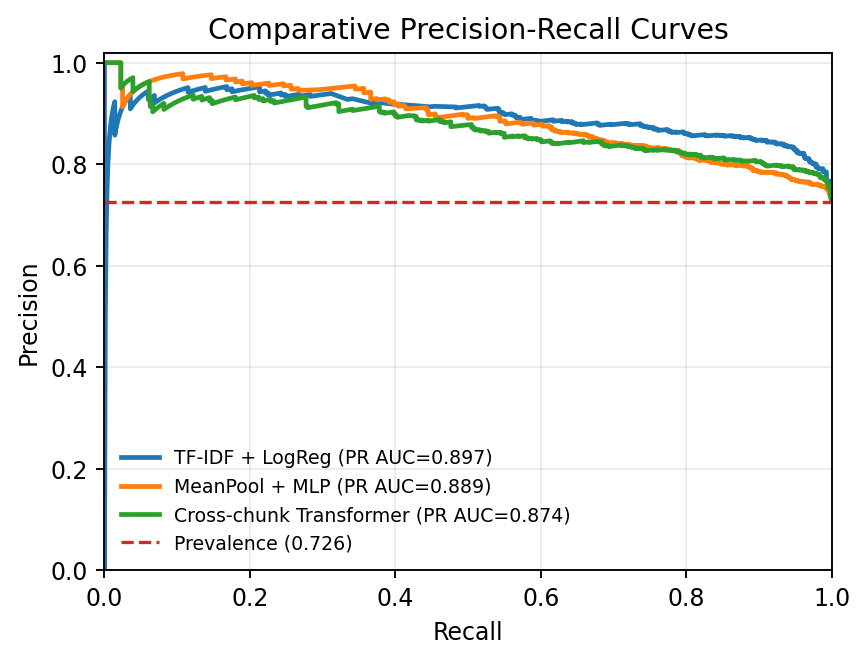
\includegraphics[width=0.94\linewidth]{figures/pr_curve_cv.png}
  \caption{Curvas comparativas de precisión-exhaustividad a partir de predicciones agregadas fuera de pliegue para la línea base léxica más sólida (TF--IDF + regresión logística), la mejor línea base densa con promedio (Promedio + MLP) y el transformer entre fragmentos. La línea horizontal discontinua marca la prevalencia positiva ($\pi \approx 0.726$). TF--IDF muestra en general el mejor compromiso entre precisión y exhaustividad, mientras que ambos modelos basados en LLM permanecen sustancialmente por encima de la referencia sin capacidad predictiva.}
  \label{fig:pr}
\end{figure}

\begin{figure}[t]
  \centering
  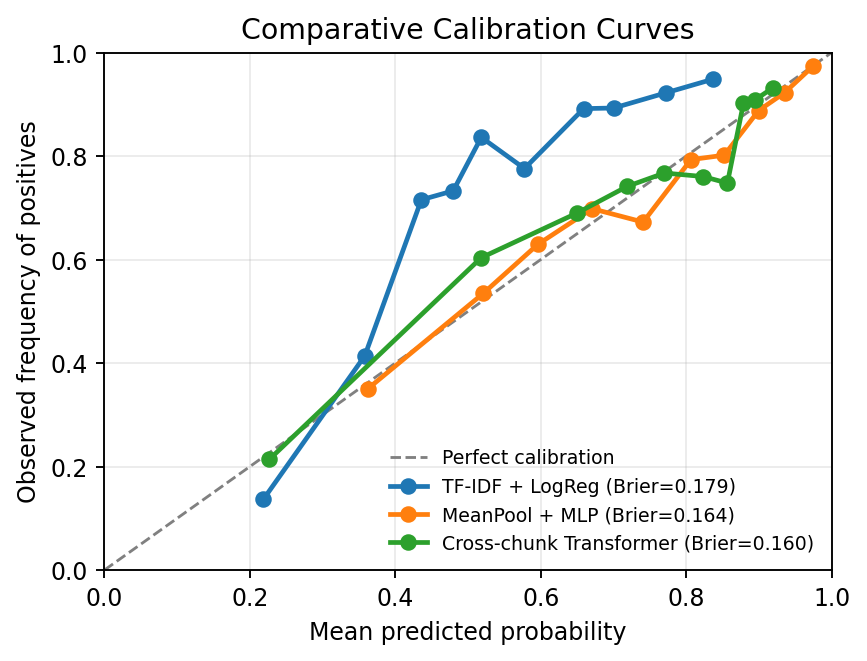
\includegraphics[width=0.94\linewidth]{figures/calibration_curve_cv.png}
  \caption{Curvas comparativas de calibración a partir de predicciones agregadas fuera de pliegue para TF--IDF + regresión logística, Promedio + MLP y el transformer entre fragmentos. La diagonal representa la calibración perfecta. El ordenamiento y la calibración no coinciden: el transformer se mantiene más próximo a una señal probabilística útil y calibrada, mientras que TF--IDF es más sólido como modelo de ordenamiento que como estimador de probabilidades.}
  \label{fig:calibration}
\end{figure}

\begin{figure}[t]
  \centering
  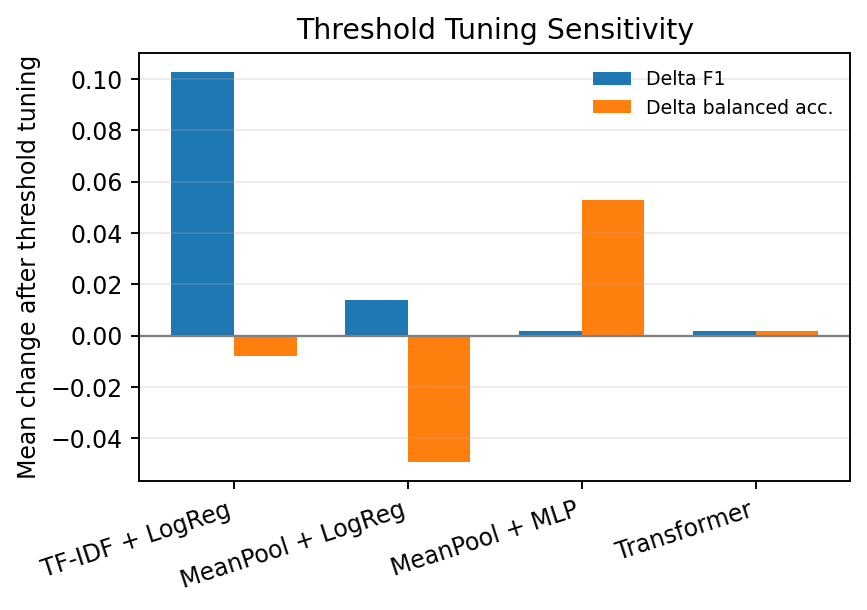
\includegraphics[width=0.94\linewidth]{figures/threshold_sensitivity_comparison.png}
  \caption{Cambio medio en F1 y exactitud balanceada del pliegue de prueba después de sustituir el umbral predeterminado de $0.5$ por el umbral que maximiza F1 en una partición interna de validación. El ajuste mejora considerablemente el F1 de TF--IDF + regresión logística, presenta efectos mixtos en los modelos con promedio y apenas modifica el transformer entre fragmentos, lo que indica una mayor estabilidad del punto operativo.}
  \label{fig:threshold-sensitivity}
\end{figure}

\chapter{Discusión}
El hallazgo principal no es que una representación domine universalmente a las demás, sino que diferentes representaciones parecen capturar distintos aspectos de la tarea. TF--IDF más regresión logística ofrece el mejor ordenamiento, lo que sugiere que la señal léxica es muy informativa en este dominio. Esto es plausible porque los documentos de licitación suelen contener fórmulas administrativas repetidas, requisitos estandarizados, terminología específica y expresiones procedimentales que pueden correlacionarse fuertemente con los resultados posteriores. En este contexto, características léxicas dispersas pueden recuperar gran parte de la señal predictiva mediante un modelo lineal relativamente simple.

Esto no debe interpretarse como evidencia contraria a las representaciones basadas en LLM. Todos los modelos no triviales de esta familia permanecen claramente por encima de las líneas base y los embeddings promediados se mantienen próximos al transformer. Ello indica que los embeddings congelados de los fragmentos ya codifican información densa útil. En otras palabras, buena parte del valor del LLM puede residir en la propia representación, más que en la complejidad del mecanismo posterior de agregación.

La comparación entre el promedio y el transformer resulta especialmente informativa. Si las interacciones detalladas entre fragmentos fueran la principal fuente de capacidad predictiva, el transformer debería dominar claramente las líneas base agregadas. Eso no ocurre en los experimentos actuales. El MLP con promedio se aproxima al transformer en ordenamiento y la regresión logística con promedio incluso lo supera en exactitud balanceada. Esto sugiere que el modelado explícito de interacciones aún no proporciona una ventaja clara de ordenamiento bajo el régimen de datos y la señal de supervisión actuales.

No obstante, el transformer conserva una ventaja importante: la calibración y la estabilidad del umbral. Obtiene el mejor puntaje de Brier y muestra muy poca sensibilidad al ajuste del umbral, mientras que TF--IDF más regresión logística se beneficia considerablemente de dicho ajuste en F1. Desde una perspectiva aplicada, esto importa porque el modelo preferido para ordenar no necesariamente es el mismo que se prefiere para priorizar mediante probabilidades o para lograr un comportamiento estable en producción. La naturaleza relativamente estandarizada de los documentos de construcción vial también puede contribuir al buen desempeño de las líneas base léxicas.

Parte de la señal predictiva puede reflejar la complejidad documental, las prácticas institucionales de redacción, la estandarización de procedimientos u otras regularidades textuales latentes. Estas señales son legítimas para la predicción porque están disponibles ex ante, cuando se emite el documento. Sin embargo, no deben interpretarse como causas de los resultados de una contratación.

En conjunto, la comparación resulta informativa incluso sin un único ganador dominante. Para aplicaciones de gobierno y democracia electrónicos, este es precisamente el punto: los sistemas de monitoreo de contrataciones requieren más que un puntaje alto de ordenamiento. También necesitan probabilidades calibradas, líneas base transparentes y umbrales cuyo comportamiento pueda explicarse antes de utilizarlos para priorizar la atención humana. Los resultados muestran que los modelos léxicos son muy competitivos, que los embeddings congelados de LLM ya capturan gran parte de la señal densa útil y que la principal ventaja comparativa del transformer reside en su calibración y estabilidad ante el umbral, no en su desempeño bruto de ordenamiento.

\chapter{Limitaciones}
Varias limitaciones deben matizar la interpretación de los resultados. En primer lugar, el conjunto supervisado es un subconjunto procesado y no una muestra representativa de toda la población de contrataciones. La inclusión exigía disponibilidad documental, extracción exitosa del texto, generación exitosa de embeddings y uno de los dos estados finales definidos. Como el filtrado se debió principalmente a restricciones de tiempo y presupuesto de procesamiento, las conclusiones deben entenderse como aplicables al subconjunto procesado.

En segundo lugar, el subconjunto procesado presenta menos desbalance que la población real. Los datos experimentales contienen alrededor de $73\%$ de ejemplos positivos, mientras que la población general está mucho más inclinada hacia resultados exitosos, con aproximadamente $94\%$ de positivos. Esta diferencia importa porque las métricas dependientes del umbral y las interpretaciones sensibles a la prevalencia no son invariantes al balance de clases. Los puntos operativos informados no deben considerarse directamente desplegables sin recalibrarlos en el entorno objetivo.

En tercer lugar, la falta de transferibilidad del umbral es una preocupación práctica. Los umbrales optimizados en validación mejoran algunas métricas de la muestra actual, especialmente para TF--IDF más regresión logística, pero pueden cambiar bajo otras prevalencias, contextos institucionales o supuestos sobre el costo de los errores. Por tanto, el ajuste debe interpretarse como una herramienta de análisis para este conjunto y no como una prescripción universal.

En cuarto lugar, la principal preocupación residual no es una fuga directa de información sobre el resultado final. Como los documentos se producen durante la convocatoria, tal fuga parece poco probable. Los riesgos más relevantes son las correlaciones predictivas indirectas, el aprendizaje de atajos, la representatividad limitada y el desajuste de distribución. Por ejemplo, los modelos podrían aprovechar regularidades institucionales o estilísticas predictivas en este conjunto, pero menos estables entre organismos, períodos o categorías de contratación. Los hallazgos también pueden ser específicos de la construcción vial y no transferirse sin cambios a otras categorías.

\chapter{Conclusión}
Este trabajo presentó un estudio comparativo de representaciones léxicas y basadas en LLM para predecir resultados de contrataciones públicas a partir de documentos de licitación. Los resultados muestran que estos documentos contienen una señal predictiva considerable, pero también que el modelo con mejor ordenamiento en la configuración actual es una línea base léxica clásica: TF--IDF más regresión logística. Al mismo tiempo, el transformer entre fragmentos sobre embeddings de LLM alcanza la mejor calibración y la mayor estabilidad ante cambios del umbral.

La comparación también indica que gran parte de la señal densa útil ya está presente en los embeddings congelados, dado que las líneas base con promedio se mantienen próximas al transformer. Esto sugiere que el modelado explícito de interacciones entre fragmentos no ofrece actualmente una ventaja clara de ordenamiento, aunque todavía puede aportar valor práctico mediante probabilidades más confiables y un comportamiento de decisión más estable. Los trabajos futuros deberían evaluar otros dominios de contratación y otros codificadores congelados.

La principal contribución del estudio es esta comparación empírica e interpretativa. Demuestra que las características léxicas capturan gran parte de la señal predictiva del dominio, que las representaciones densas preentrenadas continúan siendo útiles y que la calidad del ordenamiento, la calibración y la sensibilidad al umbral deben analizarse por separado. Estos hallazgos conectan la evaluación de aprendizaje automático con las necesidades de la gobernanza pública digital: antes de que las herramientas predictivas puedan respaldar la transparencia, la rendición de cuentas o la supervisión ciudadana de las contrataciones, sus señales, limitaciones y comportamiento operativo deben hacerse explícitos.


\clearpage
\selectlanguage{spanish}
\lhead{\emph{Referencias}}
\addcontentsline{toc}{chapter}{Referencias}
\printbibliography
\end{document}
